\documentclass[compress,12pt]{beamer}
\usepackage{xcolor}
\usepackage{tikz}

\usetheme{Arguelles}

\definecolor{bubbles}{rgb}{0.91, 1.0, 1.0}
\definecolor{cadmiumgreen}{rgb}{0.0, 0.42, 0.24}
\definecolor{forestgreen(web)}{rgb}{0.13, 0.55, 0.13}

\title{\Huge \textcolor{yellow}{MUCU}}
\subtitle{\small \textcolor{green}{Smart Automobile\\ With Automatic Navigation}}
\event{}
\date{\textcolor{bubbles}{February 4, 2024}}
\author{\textcolor{bubbles}{2005012, 2005017 \& 2005020}}
\institute{\textcolor{bubbles}{Bangladesh University of Engineering and Technology (BUET)}}

\begin{document}

\begin{frame}
  \titlepage
  \begin{tikzpicture}[remember picture, overlay]
    \node[anchor=north east, inner sep=40pt] at (current page.north east) {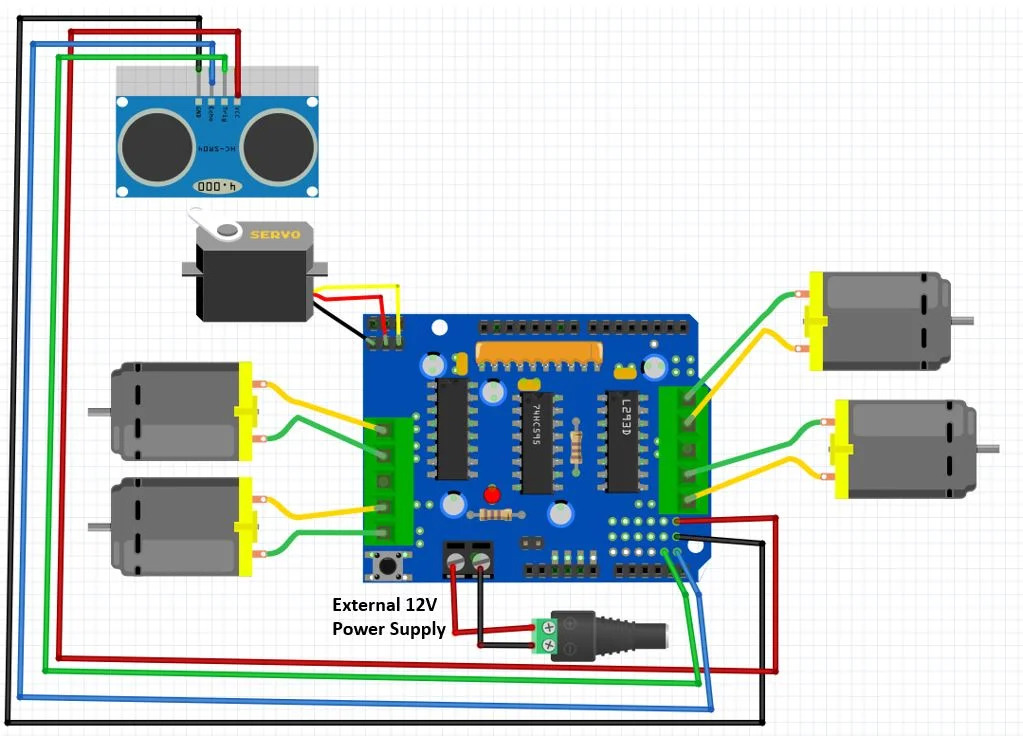
\includegraphics[scale=0.13]{Obstacle-Avoidance-Robot-connection-diagram.png}};
    \draw[white, rounded corners] ([xshift=-1mm,yshift=1mm]current page.north east) rectangle ++(2cm,-2cm);
  \end{tikzpicture}
\end{frame}

\Section{Introduction}

\begin{frame}
      \frametitle{\textcolor{cadmiumgreen}{\underline{Smart Automobile}}}
      %\framesubtitle{Subtitle here}
    A smart vehicle designed to respond to users' commands seamlessly. Besides,this intelligent marvel boasts an automatic navigation system powered by GPS. Beyond the basics, the smart car is equipped with obstacle detection mechanisms and  with additional features such as exploration capabilities and advanced security monitoring \par
      Modes of Operation:
      \begin{enumerate}[label = \roman*.]
          
            \item<1-> \textcolor{cadmiumgreen}{\textbf{Manual Mode: }}controlled by the user using {\underline{Bluetooth , voice control, etc.}}\\
            \item<2-> \textcolor{cadmiumgreen}{\textbf{Obstacle Avoiding Autonomous Mode:}} It behaves like an autonomous rover and avoids obstacles in its path.
            
            \item<3-> \textcolor{cadmiumgreen}{\textbf{GPS Navigation : }}navigates itself using \underline{GPS} and goes to destination latitude and longitude.
            
               
      \end{enumerate}
      %In all cases,the device uses ultrasonic sensor to avoid obstacles.
\end{frame}

\begin{frame}{\textcolor{cadmiumgreen}{\underline{Key Components}}}
    \begin{itemize}
        \item<1-> [-] Arduino Uno
        \item<2-> [-] Geared Motor
        \item<3-> [-] Servo Motor
        \item<4-> [-] Ultrasonic Sensor
        \item<5-> [-] GPS Module
        \item<6-> [-] Motor Driver Shield
        \item<7-> [-] Bluetooth Module
        \item<8-> [-] Camera Module
        \item<9-> [-] Wi-fi Module for live streaming
    \end{itemize}
\end{frame}

\begin{frame}{\textcolor{cadmiumgreen}{\underline{Why Arduino}}}
    \begin{itemize}
        \item<1-> [-] Need libraries for gps and bluetooth modules
        \item<2-> [-] Extensive parsing of gps data 
        \item<3-> [-] Need driver chip for accurate rotation of servo motor
        \item<4-> [-] Need accurate libraries for handling camera
        \item<5-> [-] To make the overall project compact and portable
    \end{itemize}
\end{frame}

\begin{frame}{\textcolor{cadmiumgreen}{\underline{Features}}}
    \begin{itemize}
        \item<1-> [-] Obstacle Detection
        \item<2-> [-] Automatic Path finding
        \item<3-> [-] Location Tracking
        \item<4-> [-] Transport-Delivery Services
        \item<5-> [-] Remote Exploration
        \item<6-> [-] Real Time Surveillance
    \end{itemize}
\end{frame}

\end{document}
